% =====================================================================
%  ECONSCHOOL — PROBLEMS SHEET
%  One solved problem (with a TikZ figure) + one near-twin exercise.
%
%  Compile:  pdflatex cobb-douglas.tex   (run twice for the footer)
%  No font installation needed: text and maths are Computer Modern
%  (Latin Modern where available), the same maths face the site renders
%  with KaTeX.
% =====================================================================
\documentclass[11pt]{article}

% ---- Fonts ----------------------------------------------------------
% Latin Modern if available (it is on MacTeX); base Computer Modern
% otherwise. Either way the maths face is Computer Modern.
\IfFileExists{lmodern.sty}{\usepackage[T1]{fontenc}\usepackage{lmodern}}{}

% ---- Core packages --------------------------------------------------
\usepackage{amsmath,amssymb}
\usepackage[a4paper,top=2.3cm,bottom=2.4cm,left=2.6cm,right=2.6cm]{geometry}
\usepackage{graphicx}
\usepackage{xcolor}
\usepackage{microtype}
\usepackage{enumitem}

% ---- Figures --------------------------------------------------------
\usepackage{tikz}
\usepackage{pgfplots}
\pgfplotsset{compat=1.18}
\usetikzlibrary{arrows.meta}

% ---- Layout ---------------------------------------------------------
\setlist[enumerate]{leftmargin=1.6em,itemsep=0.35em,topsep=0.3em}
\setlist[itemize]{leftmargin=1.6em,itemsep=0.2em,topsep=0.2em}
\setlength{\parindent}{0pt}
\setlength{\parskip}{0.6em}
\linespread{1.05}

% ---- Brand palette (mirrors src/styles/global.css) ------------------
\definecolor{bg}{HTML}{FAF7F2}             % cream background
\definecolor{ink}{HTML}{2A2620}            % body text
\definecolor{inksoft}{HTML}{4A4239}        % secondary text
\definecolor{inkfaint}{HTML}{7A6F62}       % tertiary / italics
\definecolor{violet}{HTML}{5A1BA6}         % titles
\definecolor{violetsoft}{HTML}{7A4FC4}     % sub-headings
\definecolor{terracotta}{HTML}{A03A2C}     % accents, links, budget line
\definecolor{terracottasoft}{HTML}{C66B5B} % light fills
\definecolor{sage}{HTML}{8AA08A}           % dividers, guide ray
\definecolor{sagesoft}{HTML}{C8D2C0}       % footer rule
\definecolor{rule}{HTML}{E5DDD0}           % hairline rules

% ---- Figure styles --------------------------------------------------
% A small reusable set for the diagrams these sheets need. Add curve
% colours per topic (demand/supply, cost curves, ...) as required.
\pgfplotsset{
  microecon/.style={
    width=8.4cm, height=6.4cm,
    axis lines=middle,
    axis line style={-{Stealth[length=2mm]}, ink},
    tick label style={font=\footnotesize, color=inksoft},
    label style={font=\small, color=inksoft},
    every axis x label/.style={at={(ticklabel* cs:1.02)}, anchor=west},
    every axis y label/.style={at={(ticklabel* cs:1.02)}, anchor=south},
    xmin=0, ymin=0,
    tick align=outside,
    enlargelimits=false,
  },
}
\tikzset{
  indiff/.style={ink, thick},                             % indifference curve (optimal)
  indiffsoft/.style={ink, thin},                          % indifference curve (context)
  budget/.style={terracotta, thick},                      % budget line
  optimum/.style={circle, fill=violet, inner sep=1.6pt},  % optimal bundle
}

% ---- Document colour ------------------------------------------------
\color{ink}
\pagecolor{bg}        % cream page; comment out this line for white

% ---- Links ----------------------------------------------------------
\usepackage[hidelinks]{hyperref}
\hypersetup{colorlinks=true, urlcolor=terracotta, linkcolor=terracotta}

% ---- Small reusable pieces ------------------------------------------
\newcommand{\eyebrow}[1]{{\color{terracotta}\textls[110]{\scshape #1}}}
% ES mark: the logo if present, a typographic fallback otherwise.
\newcommand{\esmark}{%
  \IfFileExists{es-logo.png}
    {\raisebox{-0.34\height}{
\includegraphics[height=5mm]{es-logo.png}}}
    {{\color{violet}\fontsize{20}{20}\selectfont\scshape ES}}}
\newcommand{\sagerule}{\par\vspace{0.25em}{\color{sage}\rule{\linewidth}{0.6pt}}\par\vspace{0.15em}}
\newcommand{\heading}[1]{\par\vspace{1.1em}{\color{violet}\large\bfseries #1}\par\vspace{0.25em}}
\newcommand{\subheading}[1]{\par\vspace{0.7em}{\color{violetsoft}\bfseries #1}\par\vspace{0.1em}}
\newcommand{\MU}{\mathrm{MU}}   % upright marginal-utility symbol

% ---- Footer ---------------------------------------------------------
\usepackage{fancyhdr}
\pagestyle{fancy}
\fancyhf{}
\renewcommand{\headrulewidth}{0pt}
\renewcommand{\footrulewidth}{0.4pt}
\renewcommand{\footrule}{{\color{sagesoft}%
  \vskip-\footruleskip\vskip-\footrulewidth
  \hrule height\footrulewidth width\headwidth}}
\fancyfoot[L]{\color{inkfaint}\footnotesize econschool.in}
\fancyfoot[C]{\color{inkfaint}\footnotesize\thepage}
\fancyfoot[R]{\color{inkfaint}\footnotesize youtube.com/@econ.school}

% =====================================================================
\begin{document}

% ---------- Masthead -------------------------------------------------
\noindent
\begin{tabular*}{\linewidth}{@{}l@{\extracolsep{\fill}}r@{}}
  \eyebrow{To go with the lectures} & \esmark
\end{tabular*}
\sagerule

% ---------- Title (replace per sheet) --------------------------------
{\color{violet}\fontsize{26}{30}\selectfont Cobb--Douglas\par}
\vspace{0.2em}
{\color{inkfaint}\itshape Consumer theory \;\textperiodcentered\; Problem~3
 \quad\textperiodcentered\quad
 Video: \href{https://youtu.be/SsDJB3uKrfw}{youtu.be/SsDJB3uKrfw}\par}
\sagerule

% =====================================================================
\heading{Solved problem}

A student splits a monthly allowance between food and outings. Writing
\begin{itemize}
  \item $x$: food, at price $p_x$;
  \item $y$: outings, at price $p_y$,
\end{itemize}

tastes are Cobb--Douglas, $u(x,y)=x^\alpha y^\beta$ with $\alpha,\beta>0$. With a budget of $M$ dollars, find the demand functions $x^d(p_x,p_y,M)$ and $y^d(p_x,p_y,M)$. Then illustrate the choice for $\alpha=2$, $\beta=1$, $p_x=p_y=2$ and a \$12 budget.

\subheading{Solution}
The student solves
\[
  \begin{aligned}
    \max_{(x,y)\in\mathbb{R}^2_{++}}\quad & x^\alpha y^\beta\\
    \text{s.t.}\quad & p_x x + p_y y \le M.
  \end{aligned}
\]

The student wants some of both goods, so the best bundle is interior. There the indifference curve just touches the budget line, which means the marginal rate of substitution equals the price ratio:
\[
  \mathrm{MRS}=\frac{\MU_x}{\MU_y}
  =\frac{\alpha x^{\alpha-1}y^{\beta}}{\beta x^{\alpha}y^{\beta-1}}
  =\frac{\alpha\,y}{\beta\,x}
  =\frac{p_x}{p_y}.
\]

Rearranged, this says $\beta\,p_x x=\alpha\,p_y y$: the money spent on food and the money spent on outings stand in the ratio $\alpha:\beta$. The budget binds, $p_x x+p_y y=M$, so each share is a fixed slice of the budget,
\[
  p_x\,x^d=\frac{\alpha}{\alpha+\beta}\,M,
  \qquad
  p_y\,y^d=\frac{\beta}{\alpha+\beta}\,M,
\]
which gives the demand functions
\[
  x^d(p_x,p_y,M)=\frac{\alpha}{\alpha+\beta}\,\frac{M}{p_x},
  \qquad
  y^d(p_x,p_y,M)=\frac{\beta}{\alpha+\beta}\,\frac{M}{p_y}.
\]

So the student always spends the constant fractions $\tfrac{\alpha}{\alpha+\beta}$ and $\tfrac{\beta}{\alpha+\beta}$ of the budget on the two goods, whatever the prices or income are.

With $\alpha=2$, $\beta=1$, $p_x=p_y=2$ and $M=12$ the shares are $\tfrac23$ and $\tfrac13$, so
\[
  x^d(2,2,12)=\frac{2}{3}\cdot\frac{12}{2}=4,
  \qquad
  y^d(2,2,12)=\frac{1}{3}\cdot\frac{12}{2}=2,
\]
that is $(x^\star,y^\star)=(4,2)$: \$8 on food and \$4 on outings.

\begin{center}
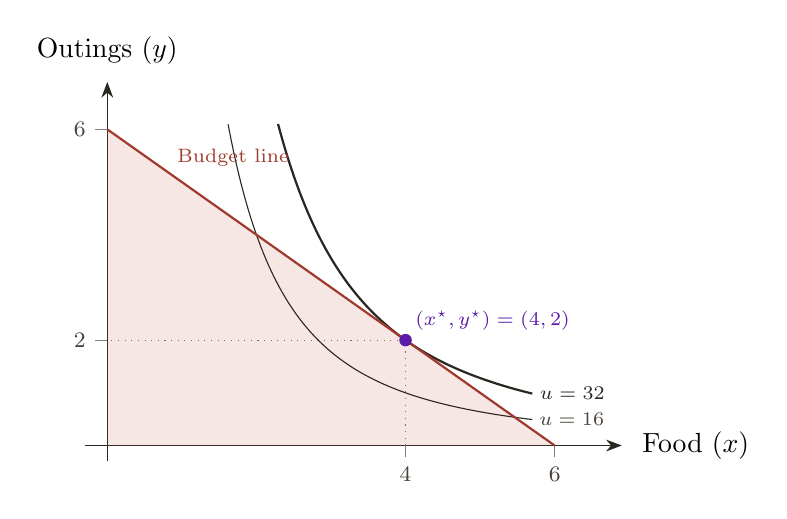
\begin{tikzpicture}
  \begin{axis}[
      microecon,
      xmin=-0.3, xmax=6.9, ymin=-0.3, ymax=6.9,
      xlabel={Food ($x$)}, ylabel={Outings ($y$)},
      xtick={4,6}, ytick={2,6},
      clip mode=individual,
  ]
    % Budget set: affordable triangle (0,0)-(6,0)-(0,6)
    \addplot[draw=none, fill=terracottasoft, fill opacity=0.16]
      coordinates {(0,0) (6,0) (0,6)} \closedcycle;

    % Lower indifference curve for context: u = 16, y = 16/x^2
    \addplot[indiffsoft, domain=1.62:5.7, samples=120] {16/(x^2)}
      node[pos=1, right=-1pt, font=\scriptsize, text=inksoft] {$u=16$};

    % Optimal indifference curve: u = x^2 y = 32, y = 32/x^2
    \addplot[indiff, domain=2.29:5.7, samples=120] {32/(x^2)}
      node[pos=1, right=-1pt, font=\scriptsize, text=ink] {$u=32$};

    % Budget line: 2x + 2y = 12  =>  x + y = 6
    \addplot[budget, domain=0:6] {6 - x}
      node[pos=0.14, above right=-1pt, font=\scriptsize, text=terracotta] {Budget line};

    % Optimum at the tangency (4, 2)
    \draw[inkfaint, dotted] (axis cs:4,0) -- (axis cs:4,2) -- (axis cs:0,2);
    \node[optimum] (opt) at (axis cs:4,2) {};
    \node[font=\scriptsize, anchor=south west, text=violet] (optlabel)
      at (axis cs:4,2) {$(x^\star,y^\star)=(4,2)$};
  %  \draw[-{Stealth[length=1.5mm]}, violet, thin] (optlabel.south west) -- (opt);
  \end{axis}
\end{tikzpicture}
\end{center}
\vspace{-0.2em}
{\color{inkfaint}\footnotesize\itshape
 Figure~1.\enspace With Cobb--Douglas tastes the indifference curves are smooth
 and convex. The student climbs to the highest curve the budget
 allows, where it just touches the budget line. At that tangency the spending on
 each good is a fixed fraction of the budget --- here $\tfrac23$ on food and
 $\tfrac13$ on outings --- giving $(x^\star,y^\star)=(4,2)$.\par}
\sagerule

% =====================================================================
\heading{Exercise}

A household buys grain and vegetables. It needs a guaranteed minimum of each before anything else --- $\gamma_x$ of grain and $\gamma_y$ of vegetables --- and beyond those floors its tastes are Cobb--Douglas. Writing
\begin{itemize}
  \item $x$: grain, at price $p_x$;
  \item $y$: vegetables, at price $p_y$,
\end{itemize}

the household's tastes are Stone--Geary,
\[
  u(x,y)=(x-\gamma_x)^\alpha\,(y-\gamma_y)^\beta,
  \qquad \alpha,\beta>0,\quad \gamma_x,\gamma_y\ge 0,
\]
defined for $x\ge\gamma_x$ and $y\ge\gamma_y$. The budget is $M$ dollars, with $M>p_x\gamma_x+p_y\gamma_y$ so that the floors are affordable.

\begin{enumerate}
  \item Find the demand functions $x^d(p_x,p_y,M)$ and $y^d(p_x,p_y,M)$. \emph{Hint:} let $\tilde x=x-\gamma_x$ and $\tilde y=y-\gamma_y$; the problem becomes Cobb--Douglas in $\tilde x,\tilde y$ with the leftover budget $M-p_x\gamma_x-p_y\gamma_y$.

  \item Take $\alpha=2$, $\beta=1$, $\gamma_x=1$, $\gamma_y=2$, $p_x=p_y=2$ and $M=12$. Find the optimal bundle, and compare it with the Cobb--Douglas answer $(4,2)$ from the solved problem.
\end{enumerate}

\subheading{Extension: shares are no longer constant}

\begin{enumerate}
  \setcounter{enumi}{2}
  \item Using your demand function $x^d$ from part~1, show that a one-dollar rise in income $M$ raises spending on grain by the fixed amount $\tfrac{\alpha}{\alpha+\beta}$, yet the \emph{share} of total spending that goes to grain still changes with $M$. Find that share as a function of $M$ and show it approaches $\tfrac{\alpha}{\alpha+\beta}$ as $M\to\infty$.
\end{enumerate}

\medskip
{\color{inksoft}\emph{Checking your work.}\enspace To discuss the exercise, join
 the community forum at \href{https://econschool.in}{econschool.in}.\par}

\end{document}
